\documentclass[a4paper,12pt]{article}
\usepackage{graphicx}
\usepackage[italian]{babel}
\usepackage{hyperref}
\usepackage{booktabs}
\usepackage[table]{xcolor}
\usepackage{float}
\usepackage{biblatex}
\addbibresource{bib.bib}

\hypersetup{
pdftitle={Sanremo Forecasting: Predizione del Vincitore di Sanremo 2025 per il televoto attraverso l'analisi del sentimento},
pdfauthor={Marzia De Maina, Enrico Ferraiolo}
}

\title{Alma Mater Studiorum - Università di Bologna}
\author{\hfill Marzia De Maina - 0001194461\\Enrico Ferraiolo - 0001191698}
\date{A.A. 2024/2025}

\title{\textbf{Sanremo Forecasting:\\ Predizione del Vincitore di Sanremo 2025 per il televoto attraverso l'analisi del sentimento}}

\begin{document}
\maketitle
\thispagestyle{empty}

\clearpage
\thispagestyle{empty}
\hfill
\clearpage

\newpage
\setcounter{page}{1}
\tableofcontents
\clearpage
\section{Introduzione}
L'idea alla base del nostro progetto nasce dalla volontà di scoprire in  anticipo chi fosse il \textbf{favorito del pubblico a casa del Festival di Sanremo 2025} attraverso l'\textbf{analisi automatica del sentimento} espresso dagli utenti sui social network.\\In particolare, ci si è concentrati sull'analisi dei contenuti pubblicati su \textit{X.com} (ex Twitter), piattaforma su cui si registra un'elevata attività durante gli eventi culturali.\\Per raggiungere questo obiettivo, abbiamo costruito un dataset contenente tutti i tweet riferiti agli artisti in gara, raccolti durante la live del Festival.\\Ciascun post è stato sottoposto a \textbf{un'analisi del sentiment} tramite il modello \textit{Twitter-roBERTa-base for Sentiment Analysis} \cite{roberta-base-sentiment-analysis}, in grado di classificare ciascun post come \texttt{positive} o \texttt{negative}.
\newpage
\section{Dataset}
Il progetto si propone di analizzare i dati relativi al Festival di Sanremo 2025, focalizzandosi sull'\textbf{opinione del pubblico a casa} attraverso la piattaforma \textit{X.com}. La creazione del dataset è stata una fase cruciale, volta a garantire l'affidabilità e la completezza delle analisi successive.

\subsection{Valutazione delle Metodologie di Raccolta dei Dati}
Dopo un'accurata valutazione delle funzionalità offerte dalle API ufficiali del social network \textit{X}, è emerso che la versione gratuita presenta \textbf{limitazioni troppo stringenti} in termini di volume dei dati accessibili, frequenza delle richieste e tipo di contenuti ottenibili (ad esempio, tweet recenti). Considerando che l’accesso alle versioni a pagamento delle API fosse economicamente fuori dalla portata del nostro progetto, si è scelto di adottare una soluzione alternativa. È stato quindi realizzato uno \textit{\textbf{Scraper}}: un bot che simula il comportamento di un utente umano durante la navigazione in una pagina web, capace di estrarre in modo strutturato le informazioni di nostro interesse. L'utilizzo della libreria \textit{Selenium} \cite{selenium} ha \textbf{permesso il controllo} del browser web \textit{Chrome} (selezionato da \cite{browser_supportati}) interagendo in modo dinamico tra le pagine. Questa scelta ha consentito di raccogliere i dati pubblicamente visibili necessari alla costruzione del dataset in modo più flessibile ed efficiente ai fini didattici.

\subsubsection{Implementazione dello Scraper}
È stata creata la classe \texttt{TwitterScraper} che implementa il bot per recuperare i tweet interessati.\\
Al fine di evitare la sospensione dell'account utilizzato è stato inserito un \textbf{waiting intelligente}: prima di passare alla successiva query di ricerca viene messo in pausa l'algoritmo per un tempo che varia dagli 1 ai 4 minuti. In questo modo è stato possibile aggirare con successo i blocchi di \textit{X}.\\
Il bot \textbf{simula un utente che naviga e compie una ricerca} su \textit{X}. Infatti prima di tutto il bot deve compiere il login sul social network. Le credenziali per l'account sono inserite in un file \texttt{.env} e, se mancanti,xx l'esecuzione di scraping si interrompe.\\
Dopo aver fatto login, si passa alla fase di costruzione della \textbf{query di ricerca}, infatti il bot costruirà e cercherà una query del genere:
\begin{verbatim}
"{Artista}" since:YYYY-MM-DD until:YYYY-MM-DD
\end{verbatim}
A questo punto il bot si ritroverà in una schermata dove sono presenti i tweet ricercati. Il bot scrollerà la pagina fino a un massimo di 15 volte (oppure finché non raccoglie \texttt{max\_tweets} (variabile che permette di definire un limite massimo di tweet da recuperare) caricando nuovi tweet.\\
I tweet vengono individuati attraverso la ricerca dell'elemento HTML \texttt{<article>} con \textit{data-testid="User-Name"}, per essere sicuri che sia stato postato da un utente. Del tweet trovato vengono salvati:
\begin{itemize}
    \item[-] Artista della query di ricerca
    \item[-] Timestamp
    \item[-] Testo del tweet
\end{itemize}
Vengono quindi selezionati i tweet contenenti solo testo.
Per ogni serata del Festival viene creata una cartella denominata \texttt{\{NumeroSerata\}\_serata}. All’interno di essa vengono generate delle sottocartelle, ciascuna rinominata con il nome di uno degli artisti in gara durante la serata selezionata. All'interno di ogni sottocartella viene poi creato un file CSV che contiene le informazioni salvate dei tweet, nominato secondo il formato \texttt{YYYY-MM-DD\_HH-HH.csv}, dove l’intervallo orario può essere: 21-22, 22-23, 23-00 oppure 00-01. In questo modo, i tweet vengono organizzati per artista e suddivisi per fascia oraria in ciascuna serata.\\
I tweet estratti e salvati, infatti, sono anche \textbf{filtrati in base alla fascia oraria e data} in cui ricadono.\\
Un esempio della struttura di salvataggio si ha in Figura \ref{fig:esempio_struttura_cartelle_scraping}.
\begin{figure}[htbp]
    \centering
    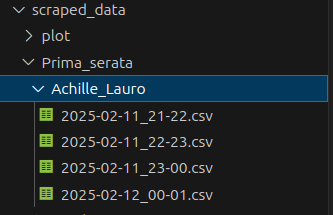
\includegraphics[width=0.5\linewidth]{media/esempio_struttura_cartelle_scraping.png}
    \caption{Esempio della struttura di salvataggio dei tweet trovati durante lo scraping}
    \label{fig:esempio_struttura_cartelle_scraping}
\end{figure}

\subsubsection{Strategia di ottimizzazione delle query di ricerca}
Durante la fase di raccolta dei dati, particolare attenzione è stata posta alla \textbf{corretta identificazione dei tweet} riferiti agli artisti partecipanti all’ultima edizione del Festival di Sanremo. Alcuni nomi di concorrenti sono nomi propri molto diffusi (come Clara, Gaia, Giorgia, Noemi) o nomi comuni (come Modà, che seppur accentato può riferirsi al mondo della moda). Questa condizione ha comportato \textbf{un alto rischio di ambiguità} e \textbf{il recupero di contenuti non pertinenti al contesto} del Festival.\\Per ovviare a questo problema, sono state definite delle query di ricerca specifiche, costruite combinando il nome dell'artista con il termine \textit{Sanremo}: "Clara Sanremo", "Gaia Sanremo", "Giorgia Sanremo", "Modà Sanremo" e "Noemi Sanremo". In questo modo è stato possibile filtrare e affinare in maniera più efficace i tweet realmente riferiti all'evento, migliorando l'accuratezza del dataset finale e riducendo il rumore informativo.

\subsubsection{Risultati dello Scraping}
Alla fine della sessione di scraping viene eseguita un'operazione di \textbf{plotting} attraverso \textit{matplotlib} per ottenere i \textbf{grafici complessivi dei tweet} ottenuti per ogni artista e per ogni serata, come si può vedere nelle Figure \ref{fig:totale_tweet_rkomi_prima_serata_fasce_orarie} e \ref{fig:totale_tweet_seconda_serata}.
\begin{figure}[htbp]
    \centering
    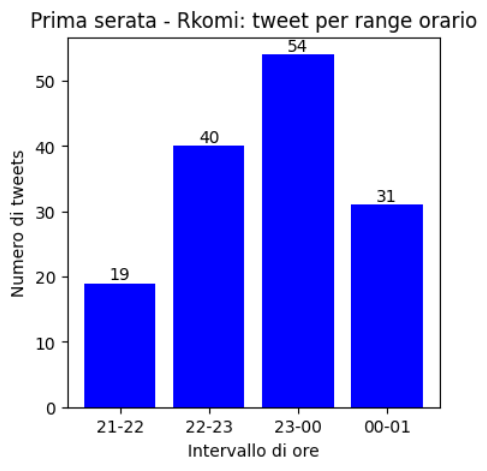
\includegraphics[width=0.5\linewidth]{media/tweet_scraped_rkomi.png}
    \caption{Tweet ottenuti per Rkomi durante lo scraping della prima serata, divisi per fasce orarie}
    \label{fig:totale_tweet_rkomi_prima_serata_fasce_orarie}
\end{figure}

\begin{figure}[htbp]
    \centering
    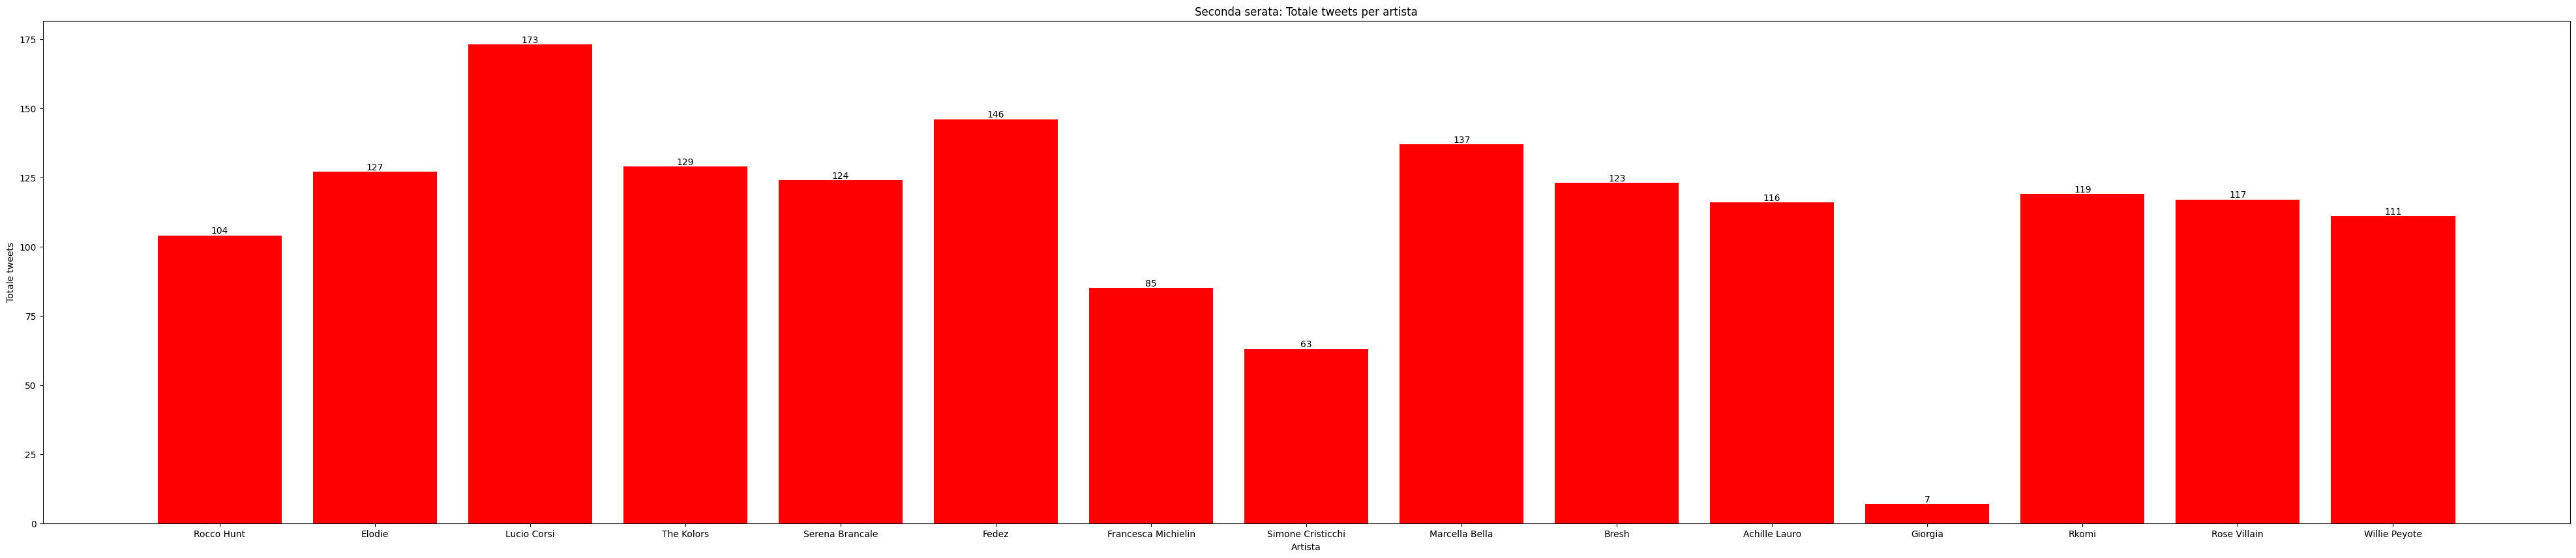
\includegraphics[width=\linewidth]{media/foto_rossa.png}
    \caption{Totale tweet per ciascun artista durante la seconda serata}
    \label{fig:totale_tweet_seconda_serata}
\end{figure}

\subsection{Pulizia del Dataset}
La fase di pulizia del dataset è stata fondamentale per assicurare l'affidabilità e la coerenza dei dati raccolti. In particolare, è stato condotto un importante intervento: \textbf{il filtraggio dei tweet non pertinenti}. Sono stati rimossi tutti quei tweet che, pur contenendo \textit{hashtag} riconducibili al Festival di Sanremo, non erano in alcun modo collegati all’evento. Questo fenomeno si verifica frequentemente a causa dell’uso improprio o strategico degli hashtag da parte degli utenti, i quali li inseriscono per aumentare artificialmente la visibilità dei propri contenuti, anche se non rilevanti. Il filtraggio è stato eseguito interamente in modo manuale.

\section{Analisi del Sentimento}
Una volta ottenuto il dataset, è stato fondamentale \textbf{analizzare il sentimento espresso in ciascun tweet} nei confronti dei singoli artisti, al fine di determinare quale fosse l'\textbf{opinione degli utenti}. Questo step si è rivelato essenziale per il raggiungimento dell’obiettivo finale, ovvero la costruzione di un \textbf{sistema in grado di valutare il sentiment del pubblico} durante il Festival.\\Per l’analisi del sentimento è stato utilizzato un modello pre-addestrato, disponibile pubblicamente e basato su \texttt{RoBERTa} \cite{roberta}, una variante ottimizzata di BERT \cite{bert} \texttt{cardiffnlp/twitter-roberta-base-sentiment-analysis} \cite{roberta-base-sentiment-analysis}.

\subsection{Scelta del Modello}
Il modello scelto è in grado di \textbf{classificare automaticamente} i testi brevi in base al \textbf{tono emotivo predominante}. È stato eseguito il fine-tuning della rete sul dataset \cite{barbieri2020tweeteval} - una raccolta di tweet (contenuto testuale) e la rispettiva \textit{label} associata, che ci permette di classificare il testo in diverse categorie di sentimento. Tuttavia, il modello scelto, \textit{cardiffnlp/twitter-roberta-base-sentiment-latest}, dato in input un tweet testuale, restituisce in output la \textbf{label di appartenenza più probabile} e la probabilità di appartenere a tale etichetta. 
Le label in cui il modello classifica del testo sono le seguenti:
\begin{itemize}
    \item[-] \texttt{Negative}
    \item[-] \texttt{Neutral}
    \item[-] \texttt{Positive}
\end{itemize}
Un esempio di output può essere il seguente:
\begin{verbatim}
    [{'label': 'Negative', 'score': 0.7236}]
\end{verbatim}
Queste sono una pool eccessiva di label, infatti delle tre totali vengono trovate di rilievo (per i fini progettuali) solamente le etichette \textbf{Negative} e \textbf{Positive}.
La probabilità totale assegnata dal modello alle label è \textit{1}: questo ci aiuta nella conversione della \textbf{classificazione} ternaria in una \textbf{binaria} tramite la ridistribuzione paritaria della percentuale da rimuovere. Nello specifico lo score della label \textbf{Neutral} va distribuito nelle altre due etichette, permettendo di ottenere risultati non ambigui per una migliore esecuzione delle fasi successive.\\
A questo punto abbiamo il necessario per \textbf{valutare ogni tweet} di cui siamo venuti in possesso attraverso lo scraping. È stato prima caricato il modello, poi eseguita la fase di inferenza per ogni tweet del dataset e infine prodotto un file csv analogo a quello descritto nella sezione precedente. Il file generato è costituito dalle seguenti colonne:
\begin{itemize}
    \item [-] \textit{Artista}
    \item [-] \textit{Datetime}
    \item [-] \textit{Contenuto}
    \item [-] \textit{Sentimento}
\end{itemize}

Per un'analisi più approfondita sono stati generati dei \textbf{grafici ausiliari} per comprendere l'analisi del sentimento dei tweet, come nelle figure \ref{fig:conteggio-sentiment-per-artista}, \ref{fig:conteggio-sentiment-per-serata} e \ref{fig:andamento-sentiment-per-serata}.

\begin{figure}[H]
    \centering
    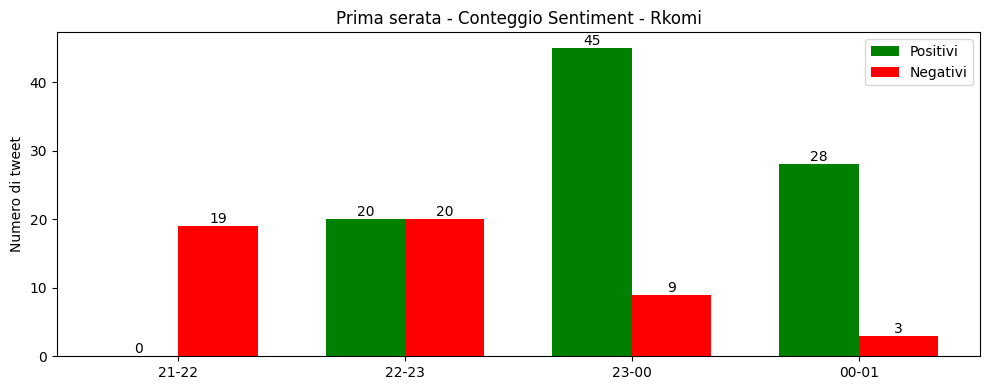
\includegraphics[width=0.8\linewidth]{media/conteggio-sentiment.png}
    \caption{Conteggio per Sentiment dei post dell'artista Rkomi durante la prima serata}
    \label{fig:conteggio-sentiment-per-artista}
\end{figure}

\begin{figure}[H]
    \centering
    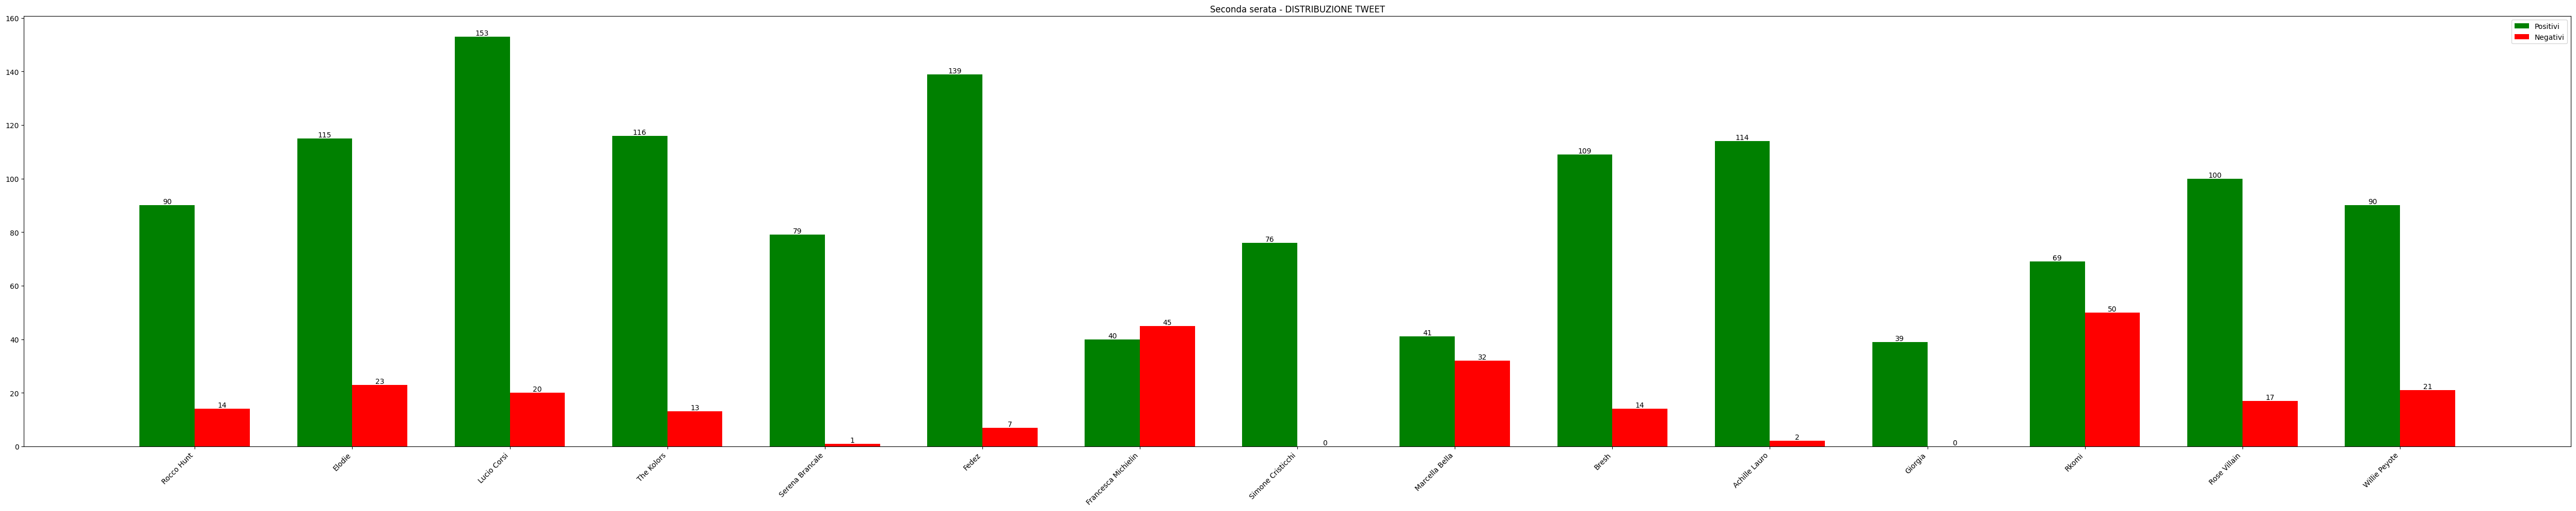
\includegraphics[width=\linewidth]{media/conteggio tweet per serata.png}
    \caption{Conteggio per Sentiment dei post di tutti gli artisti in gara durante la seconda serata}
    \label{fig:conteggio-sentiment-per-serata}
\end{figure}

\begin{figure}[H]
    \centering
    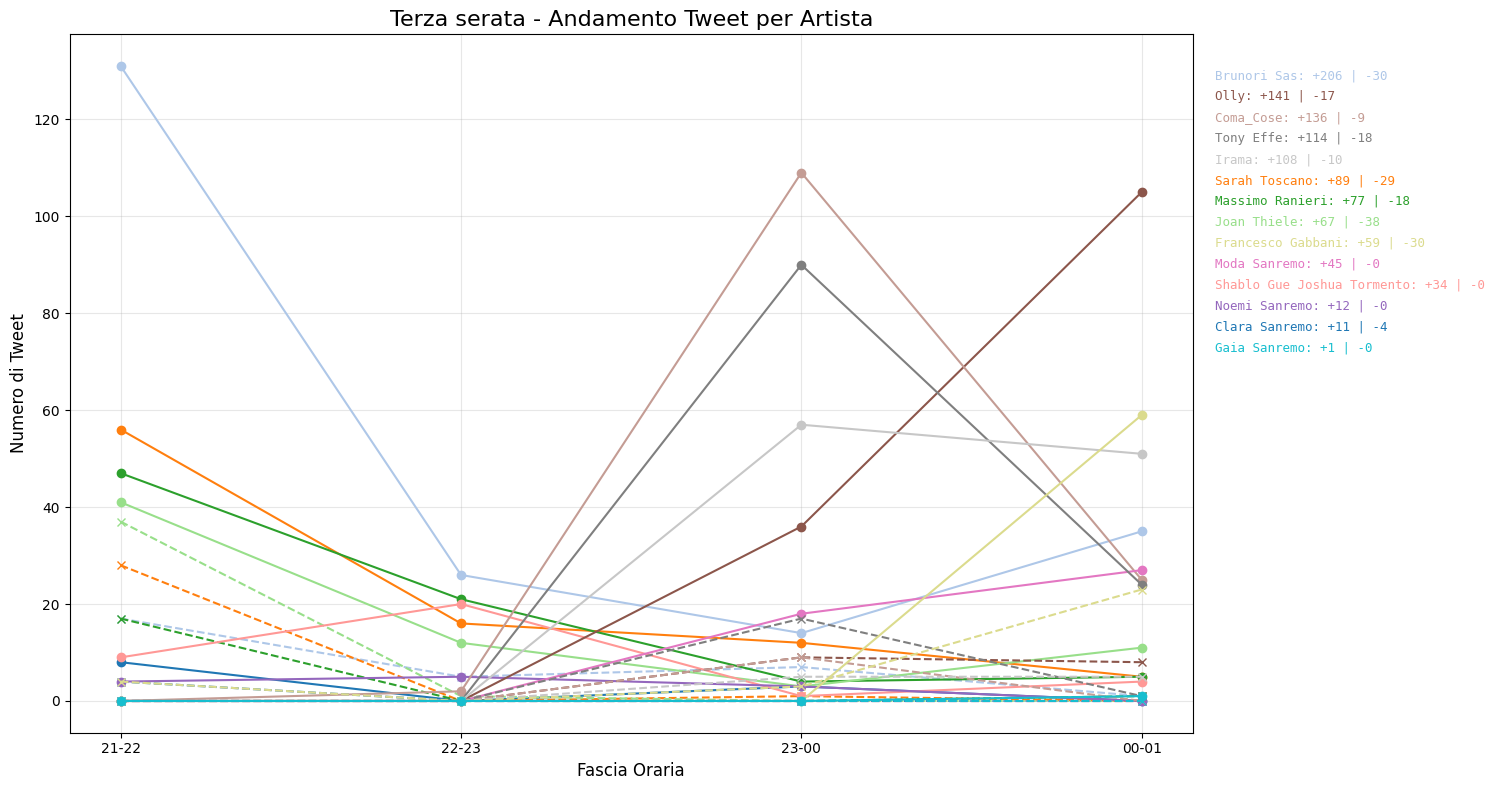
\includegraphics[width=1.2\linewidth]{media/andamento-tweet.png}
    \caption{Andamento del Sentiment per gli artisti in gara durante la terza serata}
    \label{fig:andamento-sentiment-per-serata}
\end{figure}


\section{Modello di Previsione}
L'obiettivo attuale è quello di prevedere il vincitore di Sanremo per il televoto. Prima di tutto è bene definire il problema.

\subsection{Definizione del problema}
Il progetto vuole creare uno strumento di \textit{\textbf{early prediction}} che si basa sui tweet degli utenti su \textit{X} dopo aver rilevato il sentiment per ogni post del dataset. A questo punto definiamo formalmente la situazione corrente:
\begin{enumerate}
    \item \textbf{Rilevazione del sentiment}: ogni tweet è stato classificato e ne è stato identificato il sentiment.
    \item \textbf{Aggregazione temporale}: i tweet classificati sono stati raggruppati in quattro \textbf{fasce orarie} consecutive (21-22, 22-23, 23-00, 00-01). Per ciascuna serata e per ciascun artista si ottiene così una sequenza di vettori \[(p_t,n_t)\] dove \(p_t\) è il numero di tweet positivi e \(n_t\) è il numero di tweet negativi nell'intervallo di tempo attuale \(t\).
    \item \textbf{Early prediction}: partendo dai conteggi osservati nelle finestre orarie precedenti a quella presente (\(t\)) viene costruito un modello in grado di stimare i conteggi futuri per i tweet positivi e negativi partendo dal set \[\{(p_1,n_1),...,(p_k,n_k)\}\] e quindi cercando di ottenere: \[(p_{t+1},n_{t+1})\] dove:
    \begin{itemize}
        \item [-] \textbf{\(k\)}: rappresenta il numero della \textbf{finestra oraria osservata} (ovvero di tutti i tweet già conteggiati). Quindi se \(k=1\) sto cercando di prevedere i dati della seconda finestra oraria usando come dati di input quelli della prima.
        \item [-] \textbf{\(t\)}: rappresenta la \textbf{fascia oraria attuale}, facendo un piccolo abuso di notazione possiamo definire \(t+1\) come la successiva fascia oraria. 
    \end{itemize}
È quindi chiara la correlazione tra \(t\) e \(k\): esse convivono insieme e ci permettono di definire matematicamente le finestre orarie da valutare e l'istante di tempo in cui siamo, ovvero la \textbf{finestra oraria corrente}.
    
\end{enumerate} 

\subsubsection{Previsione al Tempo \textit{t}}
Uno degli aspetti più interessanti del lavoro è la capacità di effettuare una \textbf{previsione in tempo reale} (o in differita, impostando manualmente il tempo \(t\)) sull'esito della gara, simulando scenari in cui il modello cerca di \textbf{anticipare il vincitore} in un determinato momento di una qualsiasi serata, basandosi solo sui dati disponibili fino a quell'istante (\textit{t}). Tutti i dati successivi a tale istante vengono esclusi, rendendo la previsione coerente con un contesto di \textbf{previsione parziale}. È bene notare che, avvicinandosi alla fine della gara, i dati raccolti riflettono con maggiore esattezza l'esito reale del pubblico, considerando che il modello utilizza come dati di allenamento gli \textit{n} istanti di tempo precedenti al tempo \textit{t} (\texttt{lookback}). Di conseguenza, la qualità e l'affidabilità della previsione migliorano progressivamente, fino a convergere in molti casi con l'effettivo risultato della competizione. Questo approccio consente non solo di valutare la performance del modello nel predire il vincitore finale, ma anche di esplorare la dinamica della percezione del pubblico nel corso della serata, identificando eventuali cambiamenti improvvisi o trend significativi.

\subsubsection{Implementazione}
L'istante di tempo \textit{t} viene definito dalla funzione \texttt{get\_time\_to\_predict()}:
\begin{verbatim}
    TIME_TO_PREDICT = get_time_to_predict(SERATE[-1], "23:53:00")
\end{verbatim}
che prende in input due parametri:
\begin{enumerate}
    \item La \textbf{serata} su cui effettuare la previsione (in questo caso l'ultima).
    \item L'\textbf{orario} preciso in cui effettuare la previsione (datetime).    
\end{enumerate}
La funzione \texttt{load\_data\_night()} \textbf{carica tutti i dati} dei post raccolti fino alla serata e all'orario scelti. Infine viene utilizzata la funzione \texttt{aggregate\_data()} per il raggruppamento dei dati: calcola per ogni artista il positivi e negativi. Questi dati vengono filtrati ulteriormente escludendo le fasce orarie e le serate non rilevanti e preparati per il modello tramite la funzione \texttt{prepare\_lstm\_data\_with\_labels()} che \textbf{normalizza i dati} e \textbf{codifica le etichette} degli artisti per renderli compatibili con l'apprendimento del modello. 

\subsection{Architettura del modello}
È stato costruito un \textbf{early predictor} basato su \textit{LSTM}, col fine di catturare le dinamiche temporali dei conteggi di tweet positivi e negativi restituendo così una \textit{previsione doppia} (positivi e negativi) dei conteggi futuri.\\
Il modello è costruito come segue:
\begin{itemize}
    \item [-] \textbf{Layer LSTM} da 128 unità
    \item [-] \textbf{Dropout layer} - per evitare overfitting
    \item [-] \textbf{Layer LSTM} da 64 unità
    \item [-] \textbf{Dropout layer} 
    \item [-] \textbf{Layer denso} da 64 unità intermedio che utilizza \texttt{ReLU}
    \item [-] \textbf{Dropout layer}
    \item [-] \textbf{Layer denso} da 2 unità per ottenere la previsione del conteggio di tweet positivi e negativi
\end{itemize}
Come funzione di loss è stata scelta la \textbf{MSE} poiché quello che stiamo affrontando è un problema di regressione.
Come ottimizzatore è stato scelto \textbf{Adam}.

\subsection{Training}
\subsubsection{Preparazione dei Dati}
Prima di tutto è fondamentale \textbf{aggregare i dati} per ciascun artista e intervallo orario fino a quello attuale \(t\), ottenendo così una serie temporale bidimensionale da 2 feature. Per ogni artista è stata inoltre normalizzata tale serie tramite un \textit{MiniMaxScaler} sui valori \([0,1]\), favorendo la compatibilità di comprensione e allenamento del modello.\\
Dopodiché è stata definita una \textbf{lookback window}, che serve a definire la quantità di passi temporali precedenti a quello attuale.\\
Per preservare l'ordine cronologico e la valutazione di forecasting del modello, lo split dei dati di addestramento è stato eseguito \textbf{senza shuffle} e con una frazione di dati di \textbf{validazione pari al 20\%}.\\
Per evitare l'overfitting è stata applicata la callback \textit{early stopping} sulla metrica \textit{validation loss} con una pazienza pari a 5 epoche.\\


\section{Analisi Inferenza Finale}
Dopo l'addestramento del modello si è passati alla \textbf{fase finale di inferenza} e di \textbf{valutazione dei risultati}. Abbiamo allenato il modello con i seguenti parametri per la variabile \texttt{TIME\_TO\_PREDICT = get\_time\_to\_predict(SERATE[-1], "23:53:00")}. In questo modo riusciamo a collocarci nell'ultima fascia oraria disponibile nell'ultima serata utile sia per l'inferenza che per il training del modello, ottenendo, sperabilmente, il vincitore di Sanremo per il televoto.\\
Alla fine dell'allenamento sui dati corrispondenti alla nostra posizione temporale, è stata eseguita inferenza ottenendo i risultati mostrati all'interno della Tabella \ref{tab:predizioni_post_ultima_serata} dove:
\begin{itemize}
    \item[-] \textbf{Positivo}: numero dei post predetti con sentiment positivo
    \item[-] \textbf{Negativo}: numero dei post predetti con sentiment negativo
    \item[-] \textbf{Totale}: calcolato come \(Positivo-Negativo\)
\end{itemize}

L'inferenza del modello produce \textbf{due output in floating point} che vengono troncati per simulare dei valori interi. Di conseguenza, la colonna \textit{Totale} può non coincidere esattamente con la somma dei post positivi e negativi, perché il calcolo avviene in \textbf{virgola mobile}, ma i risultati vengono mostrati come numeri interi troncati.

\begin{table}[H]
  \centering
  % Alternanza di colori per le righe
  \rowcolors{2}{gray!15}{white}
  \begin{tabular}{c l c c c}
    \toprule
    \textbf{Posizione} & \textbf{Artista} & \textbf{Totale} & \textbf{Positivi} & \textbf{Negativi} \\
    \midrule
     1 & Brunori Sas                 & 16 & 17 & 2  \\
     2 & Olly                        & 15 & 17 & 1  \\
     3 & Lucio Corsi                 & 15 & 16 & 2  \\
     4 & Fedez                       & 15 & 15 & 1  \\
     5 & Irama                       & 12 & 14 & 2  \\
     6 & Achille Lauro               & 11 & 12 & 0  \\
     7 & Bresh                       & 11 & 13 & 2  \\
     8 & Giorgia                     & 11 & 11 & 1  \\
     9 & Coma\_Cose                  & 10 & 13 & 2  \\
    10 & Rocco Hunt                  & 10 & 13 & 3  \\
    11 & Rose Villain                & 9  & 12 & 2  \\
    12 & Simone Cristicchi           & 9  & 11 & 2  \\
    13 & Tony Effe                   & 9  & 11 & 2  \\
    14 & Serena Brancale             & 9  & 9  & 0  \\
    15 & The Kolors                  & 7  & 12 & 5  \\
    16 & Elodie                      & 6  & 11 & 5  \\
    17 & Shablo Gue \& Joshua Tormento & 6  & 6  & 0  \\
    18 & Sarah Toscano               & 5  & 8  & 3  \\
    19 & Modà                        & 5  & 5  & 0  \\
    20 & Francesco Gabbani           & 5  & 7  & 2  \\
    21 & Francesca Michielin         & 5  & 9  & 4  \\
    22 & Willie Peyote               & 4  & 9  & 5  \\
    23 & Massimo Ranieri             & 4  & 6  & 2  \\
    24 & Noemi                       & 4  & 5  & 1  \\
    25 & Rkomi                       & 4  & 8  & 5  \\
    26 & Clara                       & 3  & 3  & 0  \\
    27 & Joan Thiele                 & 1  & 5  & 3  \\
    28 & Gaia                        & 1  & 1  & 0  \\
    29 & Marcella Bella              & 1  & 5  & 4  \\
    \bottomrule
  \end{tabular}
  \caption{Predizioni del numero di post per artista}
  \label{tab:predizioni_post_ultima_serata}
\end{table}

I risultati ottenuti rispecchiano, in modo quasi del tutto preciso, i risultati della \textit{CLASSIFICA GIURIA DEL TELEVOTO} di \textit{5° Serata - Sabato - Prima fase} pubblicato ufficialmente dalla RAI \cite{rai_classifiche_serate} e mostrata nella Figura \ref{fig:classifica_finale_rai}.

\begin{figure}[H]
    \centering
    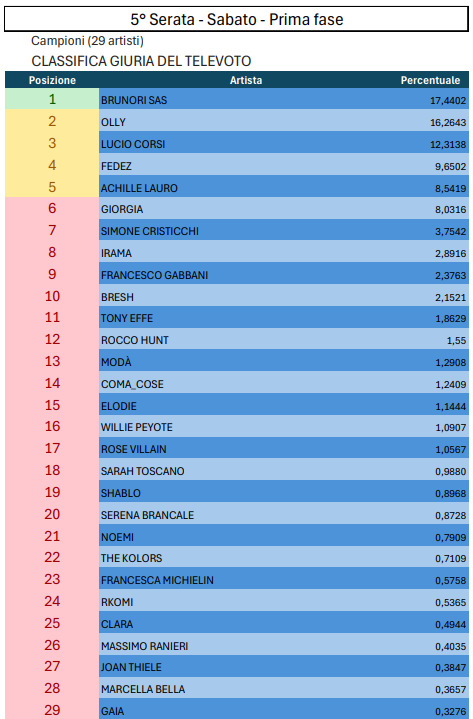
\includegraphics[width=0.7\linewidth]{media/classifica_finale_rai.png}
    \caption{\textit{CLASSIFICA GIURIA DEL TELEVOTO} di \textit{5° Serata - Sabato - Prima fase} pubblicato ufficialmente dalla RAI \cite{rai_classifiche_serate}}
    \label{fig:classifica_finale_rai}
\end{figure}

\subsection{Confronto dei Risultati}
In questa sezione vengono comparati i risultati ottenuti dal nostro modello con i risultati ufficiali. In primo luogo, l'analisi è stata effettuata \textbf{sull'intera graduatoria}, poi, in modo più accurato, \textbf{sulle prime ed ultime cinque posizioni}.
\subsubsection{Classifica Totale}
Di seguito viene riportata la Tabella \ref{tab:predizioni_post_ultima_serata_evidenza} che evidenzia le \textbf{posizioni esatte e inesatte predette dal modello} e confrontate con quelle reali in Figura \ref{fig:classifica_finale_rai}. Per comprendere a pieno i risultati del modello è stata aggiunta la colonna \textit{Errore} che evidenzia di quante posizioni si discostano i risultati ottenuti rispetto a quelli reali. Infatti, per ogni artista viene calcolato come segue:
\[Errore=PosizioneReale-PosizionePredetta\]
Si ottiene un valore \textit{positivo} se il nostro modello ha posizionato il concorrente più in alto nella tabella, \textit{negativo} se invece è più in basso.
È possibile anche studiare l'errore medio della classificazione sull'intera tabella:
\[mediaErroreTotale=\frac{80}{29}=2,75\]
L'errore medio per ogni posizione è quindi poco più di 2 posizioni.

\begin{table}[H]
  \centering
  \definecolor{verdechiaro}{RGB}{220, 255, 220}
  \definecolor{rossochiaro}{RGB}{255, 230, 230}
  \resizebox{\linewidth}{!}{%
  \begin{tabular}{c c l c c c}
    \toprule
    \textbf{Posizione} & \textbf{Errore} & \textbf{Artista} & \textbf{Totale} & \textbf{Positivi} & \textbf{Negativi} \\
    \midrule
    \rowcolor{verdechiaro}   1 & 0 & Brunori Sas                 & 16 & 17 & 2  \\
    \rowcolor{verdechiaro}   2 & 0 & Olly                        & 15 & 17 & 1  \\
    \rowcolor{verdechiaro}   3 & 0 & Lucio Corsi                 & 15 & 16 & 2  \\
    \rowcolor{verdechiaro}   4 & 0 & Fedez                       & 15 & 15 & 1  \\
    \rowcolor{rossochiaro}   5 & +3 & Irama                       & 12 & 14 & 2  \\
    \rowcolor{rossochiaro}   6 & -1 & Achille Lauro               & 11 & 12 & 0  \\
    \rowcolor{rossochiaro}   7 & +3 & Bresh                       & 11 & 13 & 2  \\
    \rowcolor{rossochiaro}   8 & -2 & Giorgia                     & 11 & 11 & 1  \\
    \rowcolor{rossochiaro}   9 & +5 & Coma\_Cose                  & 10 & 13 & 2  \\
    \rowcolor{rossochiaro}  10 & +2 & Rocco Hunt                  & 10 & 13 & 3  \\
    \rowcolor{rossochiaro}  11 & +6 & Rose Villain                & 9  & 12 & 2  \\
    \rowcolor{rossochiaro}  12 & -5 & Simone Cristicchi           & 9  & 11 & 2  \\
    \rowcolor{rossochiaro}  13 & -2 & Tony Effe                   & 9  & 11 & 2  \\
    \rowcolor{rossochiaro}  14 & +6 & Serena Brancale             & 9  & 9  & 0  \\
    \rowcolor{rossochiaro}  15 & +7 & The Kolors                  & 7  & 12 & 5  \\
    \rowcolor{rossochiaro}  16 & -1 & Elodie                      & 6  & 11 & 5  \\
    \rowcolor{rossochiaro}  17 & +2 & Shablo Gue \& Joshua Tormento & 6  & 6  & 0  \\
    \rowcolor{verdechiaro}  18 & 0 & Sarah Toscano               & 5  & 8  & 3  \\
    \rowcolor{rossochiaro}  19 & -6 & Modà                        & 5  & 5  & 0  \\
    \rowcolor{rossochiaro}  20 & -11 & Francesco Gabbani           & 5  & 7  & 2  \\
    \rowcolor{rossochiaro}  21 & +2 & Francesca Michielin         & 5  & 9  & 4  \\
    \rowcolor{rossochiaro}  22 & -6 & Willie Peyote               & 4  & 9  & 5  \\
    \rowcolor{rossochiaro}  23 & +3 & Massimo Ranieri             & 4  & 6  & 2  \\
    \rowcolor{rossochiaro}  24 & -3 & Noemi                       & 4  & 5  & 1  \\
    \rowcolor{rossochiaro}  25 & -1 & Rkomi                       & 4  & 8  & 5  \\
    \rowcolor{rossochiaro}  26 & -1 & Clara                       & 3  & 3  & 0  \\
    \rowcolor{verdechiaro}  27 & 0 & Joan Thiele                 & 1  & 5  & 3  \\
    \rowcolor{rossochiaro}  28 & +1 & Gaia                        & 1  & 1  & 0  \\
    \rowcolor{rossochiaro}  29 & -1 & Marcella Bella              & 1  & 5  & 4  \\
    \bottomrule
  \end{tabular}
  } % fine resizebox
  \caption{Classifica predizioni post con righe in evidenza e colonna Errore}
  \label{tab:predizioni_post_ultima_serata_evidenza}
\end{table}


È bene sottolineare che i risultati del modello sono ovviamente più precisi nella \textbf{Top 5} e nella \textbf{Bottom 5} della classifica, questo perché le posizioni intermedie, come si può notare dalla classifica ufficiale, hanno una ridotta differenza percentuale.

\subsubsection{Top 5 e Bottom 5}
Le seguenti tabelle riportano una sola porzione di ogni classifica precedente: più precisamente vengono visualizzate le rispettive \textit{Top 5} (Figure \ref{tab:predizioni_post_ultima_serata_top5} e \ref{tab:ultima_serata_top5_ufficiale}) e \textit{Bottom 5} (Figure \ref{tab:predizioni_post_ultima_serata_bottom5} e \ref{tab:ultima_serata_bottom5_ufficiale}).
\begin{table}[H]
  \centering
  \definecolor{verdechiaro}{RGB}{220, 255, 220}
  \definecolor{rossochiaro}{RGB}{255, 230, 230}
  \rowcolors{5}{gray!15}{white} % alternanza parte da riga 5
  \resizebox{0.8\linewidth}{!}{%
  \begin{tabular}{c l c c c}
    \toprule
    \textbf{Posizione} & \textbf{Artista} & \textbf{Totale} & \textbf{Positivi} & \textbf{Negativi} \\
    \midrule
    \rowcolor{verdechiaro}
     1 & Brunori Sas                 & 16 & 17 & 2  \\
    \rowcolor{verdechiaro}
     2 & Olly                        & 15 & 17 & 1  \\
    \rowcolor{verdechiaro}
     3 & Lucio Corsi                 & 15 & 16 & 2  \\
    \rowcolor{verdechiaro}
     4 & Fedez                       & 15 & 15 & 1  \\
    \rowcolor{rossochiaro}
     5 & Irama                       & 12 & 14 & 2  \\
    \bottomrule
  \end{tabular}
  }
  \caption{Top 5 delle predizioni effettuate dal modello}
  \label{tab:predizioni_post_ultima_serata_top5}
\end{table}

\begin{table}[H]
  \centering
  \definecolor{verdechiaro}{RGB}{220, 255, 220}
  \definecolor{rossochiaro}{RGB}{255, 230, 230}
  \rowcolors{5}{gray!15}{white} % alternanza parte da riga 5
  \resizebox{0.8\linewidth}{!}{%
  \begin{tabular}{c l c}
    \toprule
    \textbf{Posizione} & \textbf{Artista} & \textbf{Percentuale (\%)}\\
    \midrule
    \rowcolor{verdechiaro}
     1 & Brunori Sas                 & 17,4402  \\
    \rowcolor{verdechiaro}
     2 & Olly                        & 16,2643  \\
    \rowcolor{verdechiaro}
     3 & Lucio Corsi                 & 12,3138  \\
    \rowcolor{verdechiaro}
     4 & Fedez                       & 9,6502  \\
    \rowcolor{rossochiaro}
     5 & Achille Lauro                       & 8,5419  \\
    \bottomrule
  \end{tabular}
  }
  \caption{Top 5 ufficiale}
  \label{tab:ultima_serata_top5_ufficiale}
\end{table}

\begin{table}[H]
  \centering
  \definecolor{verdechiaro}{RGB}{220, 255, 220}
  \definecolor{rossochiaro}{RGB}{255, 230, 230}
  \rowcolors{5}{gray!15}{white} % alternanza parte da riga 5
  \resizebox{0.8\linewidth}{!}{%
  \begin{tabular}{c l c c c}
    \toprule
    \textbf{Posizione} & \textbf{Artista} & \textbf{Totale} & \textbf{Positivi} & \textbf{Negativi} \\
    \midrule
    \rowcolor{rossochiaro}
     25 & Rkomi                 & 16 & 17 & 2  \\
    \rowcolor{rossochiaro}
     26 & Clara                        & 15 & 17 & 1  \\
    \rowcolor{verdechiaro}
     27 & Joan Thiele                 & 15 & 16 & 2  \\
    \rowcolor{rossochiaro}
     28 & Gaia                       & 15 & 15 & 1  \\
    \rowcolor{rossochiaro}
     29 & Marcella Bella                       & 12 & 14 & 2  \\
    \bottomrule
  \end{tabular}
  }
  \caption{Bottom 5 delle predizioni effettuate dal modello}
  \label{tab:predizioni_post_ultima_serata_bottom5}
\end{table}

\begin{table}[H]
  \centering
  \definecolor{verdechiaro}{RGB}{220, 255, 220}
  \definecolor{rossochiaro}{RGB}{255, 230, 230}
  \rowcolors{5}{gray!15}{white} % alternanza parte da riga 5
  \resizebox{0.8\linewidth}{!}{%
  \begin{tabular}{c l c}
    \toprule
    \textbf{Posizione} & \textbf{Artista} & \textbf{Percentuale (\%)}\\
    \midrule
    \rowcolor{rossochiaro}
     25 & Clara                 & 0,4944  \\
    \rowcolor{rossochiaro}
     26 & Massimo Ranieri                        & 0,4035  \\
    \rowcolor{verdechiaro}
     27 & Joan Thiele                 & 0,3837  \\
    \rowcolor{rossochiaro}
     28 & Marcella Bella                       & 0,3657  \\
    \rowcolor{rossochiaro}
     29 & Gaia                       & 0,3276  \\
    \bottomrule
  \end{tabular}
  }
  \caption{Bottom 5 ufficiale}
  \label{tab:ultima_serata_bottom5_ufficiale}
\end{table}

Le tabelle evidenziano \textit{in verde i risultati uguali} e \textit{in rosso quelli sbagliati}, notiamo infatti che il nostro modello ha predetto in modo corretto \textbf{4/5 della Top 5} ufficiale del televoto, portando a un ottimo risultato.\\
Per capire a pieno i risultati del modello possiamo calcolare l'errore medio:
\[mediaErroreTop5=\frac{3}{5}=0,6\]
\[mediaErroreBottom5=\frac{4}{5}=0,8\]
Capiamo quindi che il modello nelle due \textit{mini-classifiche} sbaglia la classificazione per poco meno di una posizione.

\subsection{Grafici delle Previsioni}
Di seguito, nelle Figure \ref{fig:rose_prediction_plot} e \ref{fig:totale_prediction_plot}, vengono riportati i grafici per \textbf{l'andamento dei tweet predetti} durante l'ultima serata del Festival di Sanremo 2025.

\begin{figure}[H]
    \centering
    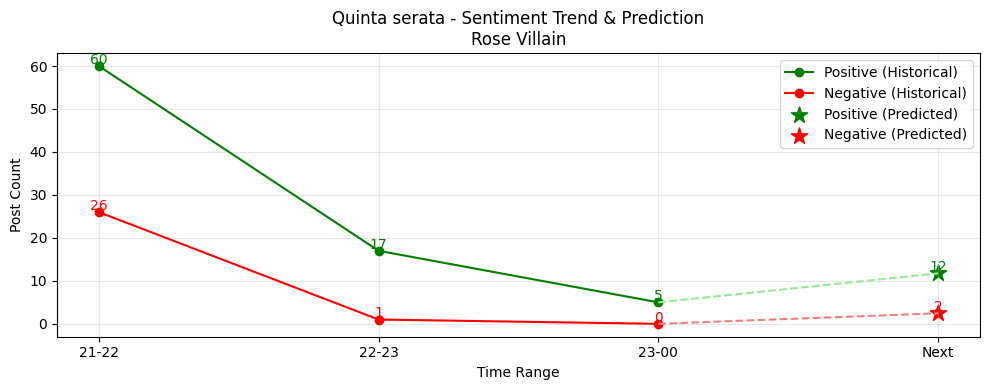
\includegraphics[width=\linewidth]{media/rose_prediction.png}
    \caption{Predizione del Sentiment per Rose Villain durante la 5° serata}
    \label{fig:rose_prediction_plot}
\end{figure}

\begin{figure}[H]
    \centering
    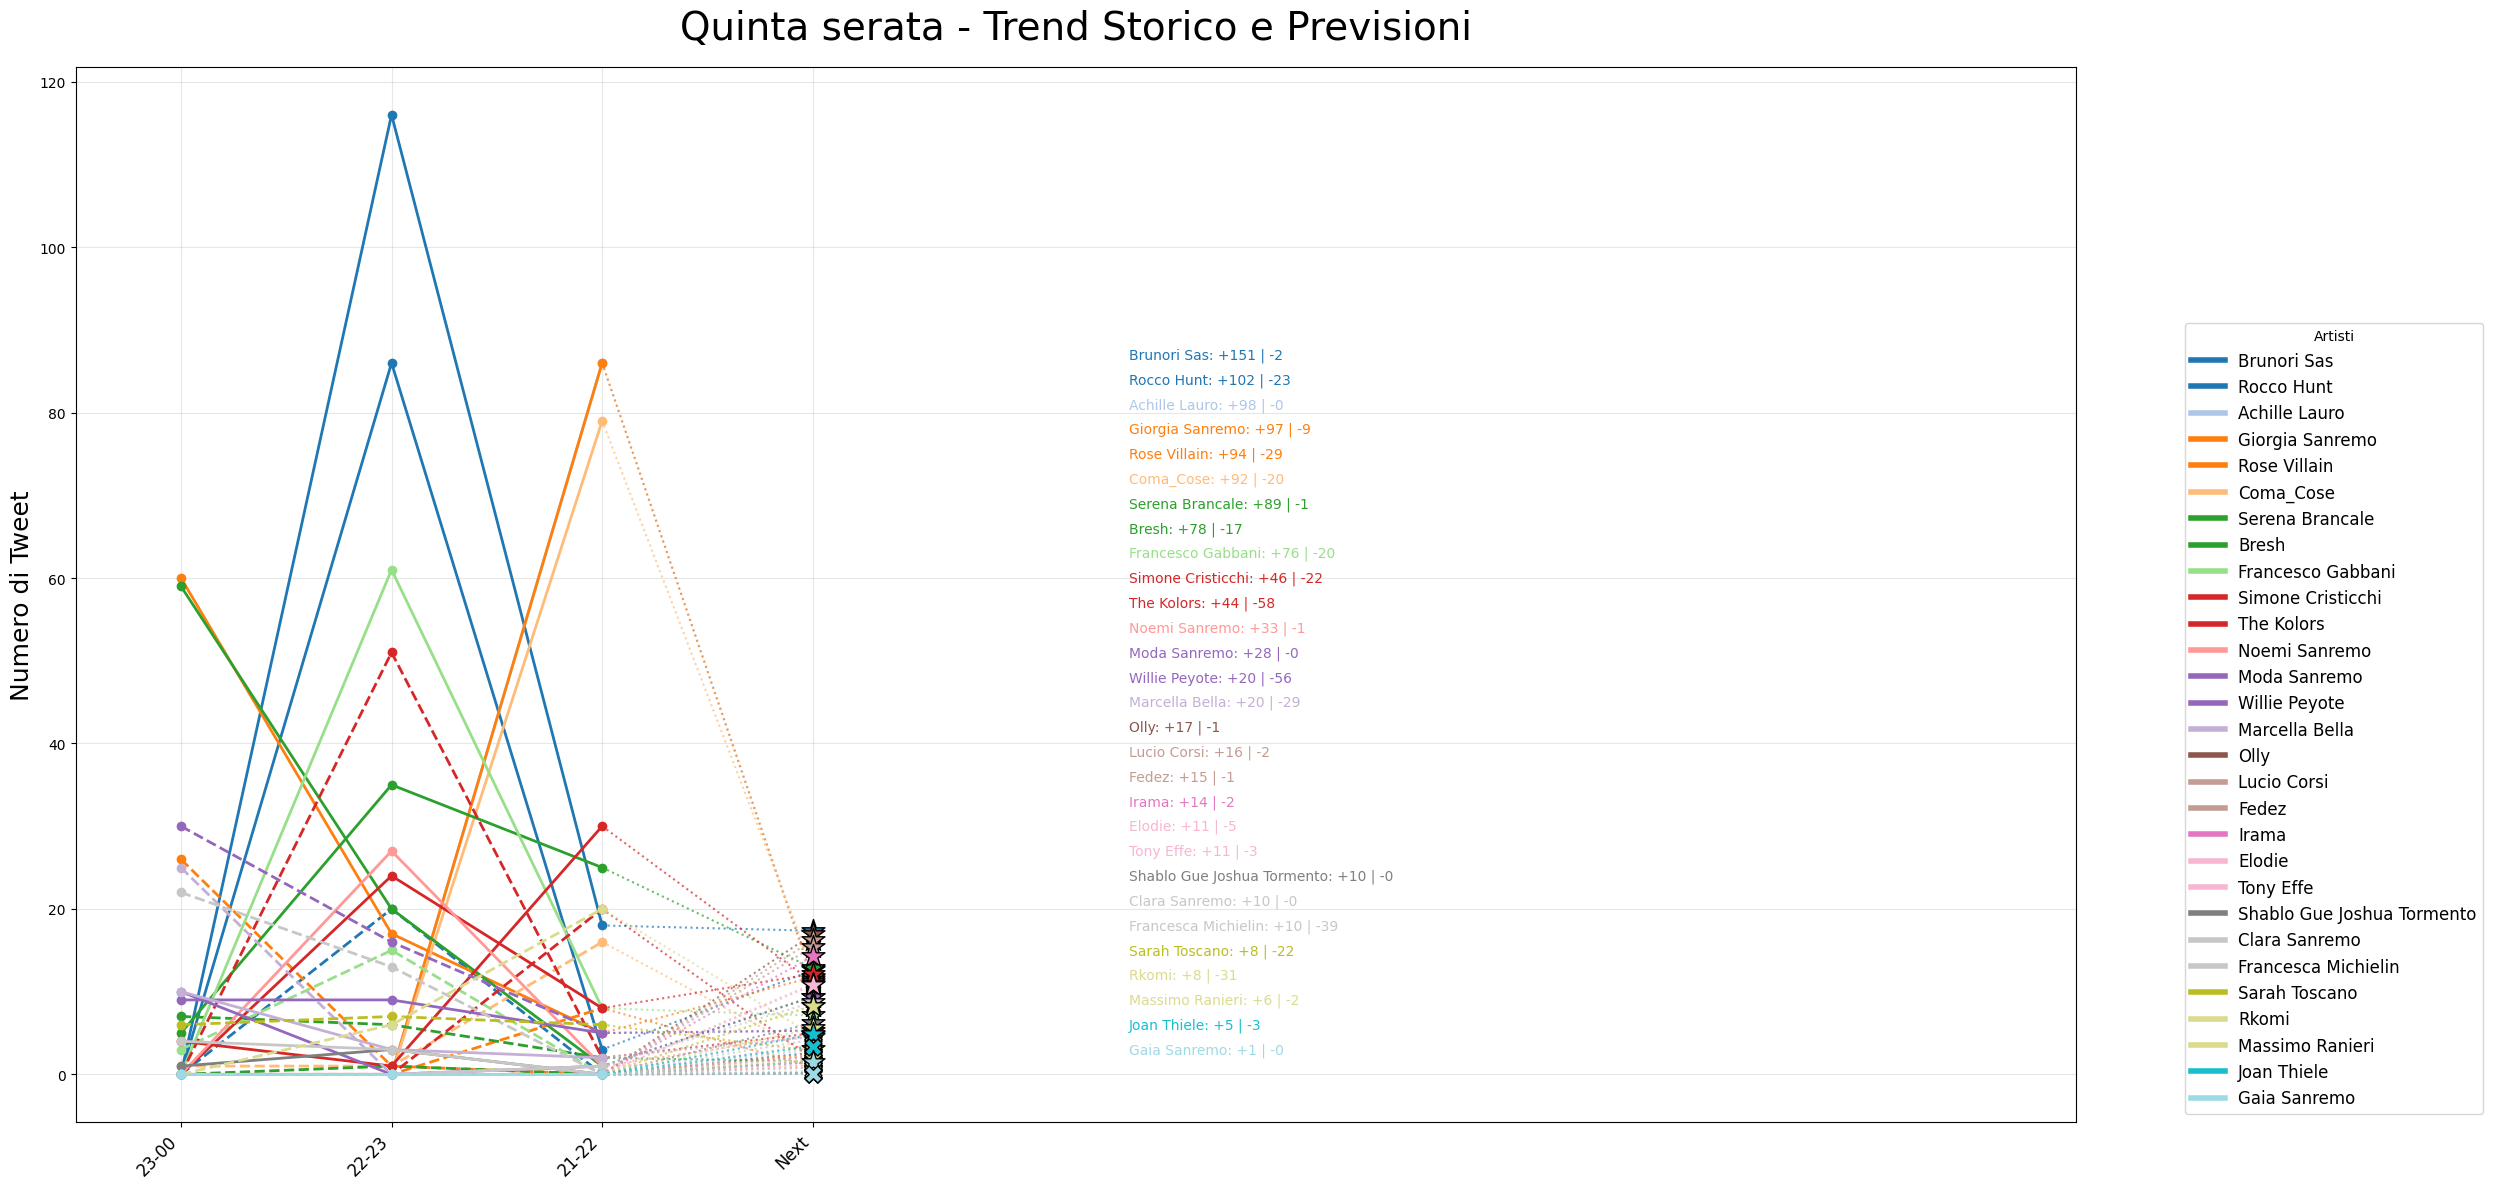
\includegraphics[width=1.2\linewidth]{media/previsioni_quintaserata.png}
    \caption{Predizione del Sentiment per ogni artista in gara durante la 5° serata}
    \label{fig:totale_prediction_plot}
\end{figure}

\newpage
\printbibliography
\thispagestyle{empty}
\end{document}
